\begin{figure}[h] 
\centering 
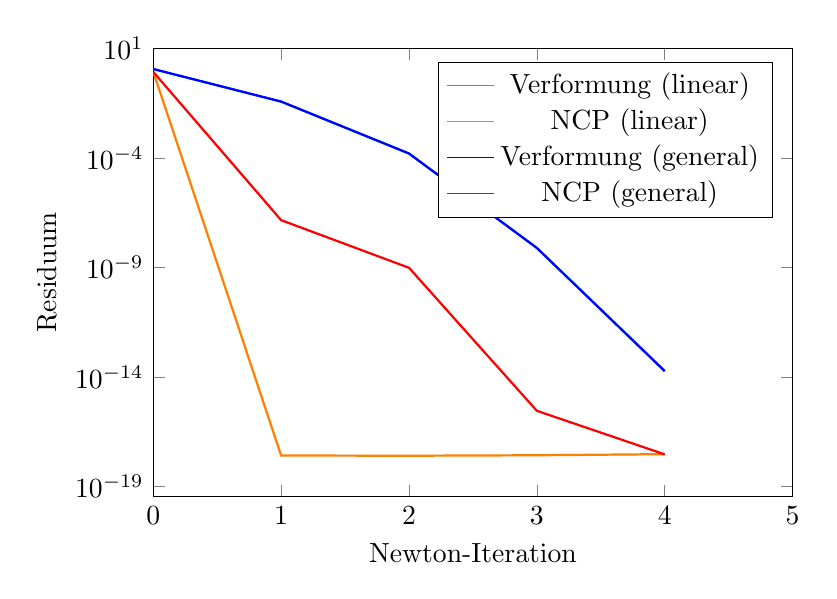
\begin{tikzpicture}[every plot/.append style={thick}] 
\begin{axis}[ 
label style={font=\normalsize}, 
xlabel={Newton-Iteration}, 
ylabel={Residuum}, 
xmin=0, xmax=5, 
ymode=log, 
ymin=0, ymax=10, 
width=0.8\textwidth, 
height=0.6\textwidth, 
legend pos=north east, 
legend style={cells={align=left}}, 
grid style=dashed, 
] 
\addplot[ 
color=cyan, 
] 
coordinates { 
(0, 1.11e+00)(1, 3.65e-02)(2, 1.56e-04)(3, 7.74e-09)(4, 1.94e-14)}; 
\addlegendentry{Verformung (linear)} 
\addplot[ 
color=orange, 
] 
coordinates { 
(0, 8.29e-01)(1, 2.65e-18)(2, 2.59e-18)(3, 2.72e-18)(4, 3.06e-18)}; 
\addlegendentry{NCP (linear)} 
\addplot[ 
color=blue, 
] 
coordinates { 
(0, 1.12e+00)(1, 3.66e-02)(2, 1.57e-04)(3, 7.73e-09)(4, 1.86e-14)}; 
\addlegendentry{Verformung (general)} 
\addplot[ 
color=red, 
] 
coordinates { 
(0, 8.24e-01)(1, 1.43e-07)(2, 9.64e-10)(3, 2.89e-16)(4, 2.99e-18)}; 
\addlegendentry{NCP (general)} 
\end{axis} 
\end{tikzpicture} 
\caption{Residuen des Stoffgesetzes 'Neo Hooke' mit Hinderniss 'Parabel' und 2178 Freiheitsgraden für die Verschiebung.} 
\label{fiq:NeoHooke_Parabel_level4} 
\end{figure} 
